\chapter{Tests and Benchmarks}\label{chap:test}
\section{Comparison of Reachability Analyzers}
In this section we evaluate our approach through various experiments.
All tests were run on a Intel Core i7-3770 CPU, \@3.4GHz with 8Gb of RAM computer.

To validate our approach, we first tested a small model, $\lambda$-phage model \cite{thieffry1995dynamical} to compare with an alternative reachability analyzer Pint \cite{pauleve2012} implementing solely analysis using SLCG \cite{pauleve2017reduction,folschette2015,pauleve2011}.
In this model with 4 automata and 12 transitions (without taking consideration of the self-regulations),
our result shows complete conclusiveness while Pint cannot (Figure \ref{fig:LCG_lambdaPhage}). %able to figure out the reachability of $cro_1$ when $cl_1$ and $cll_1$ are in the initial state (Figure \ref{fig:LCG_lambdaPhage}).
PermReach \cite{chai2018heuristic} is not able either to handle some of the special cases where multiple states of one automaton appear in different branches (Figure \ref{fig:countexPerm}).
Theses cases are solvable by ASPReach.
The whole approach is implemented in Python3\footnote{Code and testing data available at \url{https://github.com/XinweiChai/LCG-in-ASP}}.
The call of ASP is done by package \textit{pyasp}\footnote{\url{https://pypi.python.org/pypi/pyasp}}. 
%In big examples TCR and EGFR, it outputs the sequence from initial state towards final state.
%More importantly, it gives decidable reachability for any input. 

\begin{figure}[ht]
\centering
    \begin{tikzpicture}[aS]  
  	
  	\startl{cro_1};
  	\specl{above}{cro_1}{cII_0};
  	\link{cII_0}{cI_1};
  	\edl{cI_1};
  	\specl{below}{cro_1}{cI_0};
	\path (cI_0s) edge (cII_0);
    
    \end{tikzpicture}

    \caption[SLCG of $\lambda$-phage model]{One SLCG of $\lambda$-phage model, automaton $cl$ appears in both branches of the \textbf{AND gate}. Static analyzer Pint cannot decide whether in this case $cro_1$ is reachable or not, because it does not consider the order in the state sequence even though there exists a solution is of length 3: $cll_0::cl_0::cro_1$ corresponding to the trajectory $\acm{cl_1}{cll_1}{cll_0}::\acm{cll_0}{cl_1}{cl_0}::\acm{cll_0,cl_0}{cro_0}{cro_1}$.}
    \label{fig:LCG_lambdaPhage}
\end{figure}
\begin{figure}[ht]
    \centering
    \begin{tikzpicture}[aS]  
  	
	\startl{a_1};
	\specl{above}{a_1}{b_1};
	\specl{above}{b_1}{d_0};
	\edl{d_0};
	\link{b_1}{a_0};
 	\edl{a_0};
	\link{a_1}{c_1};
 	\link{c_1}{d_1};
 	\link{d_1}{c_0};
 	\edl{c_0};
 	\specl{below}{c_1}{e_0};
 	\edl{e_0};
    \end{tikzpicture}
    \caption[Counterexample of PermReach]{This counterexample shows former PermReach is inconclusive if multiple states of one automaton appear in the branches of one \textbf{AND gate} ($d_0$ and $d_1$ in this example). 
    However there exists a consistent state sequence: $d_1::b_1::c_1::a_1$ corresponding to the trajectory $\acm{c_0}{d_0}{d_1}::\acm{d_0,a_0}{b_0}{b_1}::\acm{d_1,e_0}{c_0}{c_1}::\acm{b_1,c_1}{a_0}{a_1}$ which could be found by ASPReach.}\label{fig:countexPerm}
\end{figure}

To evaluate the scalability in \textit{in silico} networks, we take T-cell Receptor model (TCR) \cite{saez2007logical} and epidermal growth factor receptor model (EGFR) \cite{samaga2009logic} as examples, with the former one containing 95 automata and 206 transitions and the latter one containing 104 automata and 389 transitions respectively. 

These models are originally Boolean networks.
According to the approach in Appendix \ref{appendix:trans}, BNs are transformed into ABANs. 
Here, we ran the same test as in \cite{folschette2015}. In the TCR model, we take 3 automata as input (\texttt{cd4 cd28 tcrlig}), varying exhaustively their initial states combinations ($2^3$), take the reachability of states of 5 automata (\texttt{sre ap1 nfkb nfat sigmab}) as output. 
Similarly we carried a bigger test on EGFR model with 13 automata %\footnote{\texttt{erbb1 erbb2 erbb3 erbb4 bir btc egf epr nrg1a nrg1b nrg2b nrg4 tgfa}}
as input and 12 automata %\footnote{\texttt{elk1 creb ap1 hsp27 actin\_reorg cmyc pro\_apoptotic p70s6\_2 pkc stat1 stat3 stat5}}
as output.
We first tested the performance of traditional model checkers, Mole\footnote{\url{http://www.lsv.fr/~schwoon/tools/mole}} and NuSMV\footnote{\url{http://nusmv.fbk.eu}}, in which Mole turns out to be memory-out for 6 in 12 outputs, and all memory-out for NuSMV in model EGFR. 
Due to the big state space, traditional model checkers are not applicable.
In the TCR tests, our approach gives exactly the same result as Pint did. 
As for EGFR tests, ASPReach returned no inconclusive output.

\begin{table}[ht]
    \begin{tabular}{|c|c|c|c|}
    \hline
     Model    &  \multicolumn{3}{c|}{$\lambda$-phage}\\
     \hline
     Inputs    & \multicolumn{3}{c|}{4}\\
     \hline
     Outputs&\multicolumn{3}{c|}{4}\\
     \hline
     Total tests&\multicolumn{3}{c|}{$2^4\times 4=64$}\\
     \hline
     Analyzer  &  Pint  &  \textbf{PermReach}   &\textbf{ASPReach}\\
     \hline
     Reachable & 36(56\%)& \multicolumn{2}{c|}{38(59\%)} \\
     \hline
     Unreachable&\multicolumn{3}{c|}{26(41\%)}\\
     \hline
     \textbf{Inconclusive} &\textcolor{red}{\textbf{2(3\%)}}&\multicolumn{2}{c|}{\textcolor{blue}{\textbf{0(0\%)}}}\\
     \hline
     Total time & \multicolumn{3}{c|}{$<1$s}\\
    \hline
     Model    &  \multicolumn{3}{c|}{TCR}\\
     \hline
     Inputs    & \multicolumn{3}{c|}{3}\\
     \hline
     Outputs&\multicolumn{3}{c|}{5}\\
     \hline
     Total tests&\multicolumn{3}{c|}{$2^3\times 5=40$}\\
     \hline
     Analyzer  &  Pint  &  \textbf{PermReach}   &\textbf{ASPReach}\\
     \hline
     Reachable & \multicolumn{3}{c|}{16(40\%)} \\
     \hline
     Unreachable&\multicolumn{3}{c|}{24(60\%)} \\
     \hline
     \textbf{Inconclusive} &\multicolumn{3}{c|}{\textcolor{blue}{\textbf{0(0\%)}}} \\
     \hline
     Total time &  7s     &0.85s  &  40s        \\
    \hline
     Model    &  \multicolumn{3}{c|}{EGFR}\\
     \hline
     Inputs    & \multicolumn{3}{c|}{13}\\
     \hline
     Outputs&\multicolumn{3}{c|}{12}\\
     \hline
     Total tests&\multicolumn{3}{c|}{$2^{13}\times 12=98,304$}\\
     \hline
     Analyzer  &  Pint  &  \textbf{PermReach}   &\textbf{ASPReach}\\
     \hline
     Reachable & 64,282(65.4\%)  & \multicolumn{2}{c|}{74,268(75.5\%)} \\
     \hline
     Unreachable&\multicolumn{3}{c|}{24,036(24.5\%)}\\
     \hline
     \textbf{Inconclusive} &\textcolor{red}{\textbf{9,986(10.1\%)}}&\multicolumn{2}{c|}{\textcolor{blue}{\textbf{0(0\%)}}}   \\
     \hline
     Total time & \textbf{9h50min}      & \textbf{15min31s}         & \textbf{3h46min} \\
     \hline
    \end{tabular}
    
    %\begin{tabular}{|c|c|c|c|c|c|c|c|c|c|}
    %\hline
  	%Model	&\multicolumn{3}{c|}{$\lambda$-phage}	&	  \multicolumn{3}{c|}{TCR} & \multicolumn{3}{c|}{EGFR}  \\
    %\hline
    %Inputs&\multicolumn{3}{c|}{4}	&	  \multicolumn{3}{c|}{3} & \multicolumn{3}{c|}{13}\\
    %\hline
    %Outputs&\multicolumn{3}{c|}{4} &	  \multicolumn{3}{c|}{5} & \multicolumn{3}{c|}{12} \\
    %\hline
    %Total tests&\multicolumn{3}{c|}{$2^4\times 4=64$} & \multicolumn{3}{c|}{$2^3\times 5=40$} & \multicolumn{3}{c|}{$2^{13}\times 12=98,304$}\\
    %\hline
    %Analyzer  &  Pint  &  \textbf{PermReach}   &\textbf{ASPReach}    &  Pint  &  \textbf{PermReach}     &\textbf{ASPReach}   &  Pint  &  \textbf{PermReach}     &\textbf{ASPReach}             \\
    %\hline
    %Reachable    & 36(56\%)& 38(59\%)& 38(59\%)   &  \multicolumn{3}{c|}{16(40\%)}  & 64,282(65.4\%)  & \multicolumn{2}{c|}{74,268(75.5\%)}\\
    %\hline
    %\textbf{Inconclusive} & \textcolor{red}{\textbf{2(3\%)}}&\multicolumn{2}{c|}{\textcolor{blue}{\textbf{0(0\%)}}}& \multicolumn{3}{c|}{0(0\%)}    &\textcolor{red}{\textbf{9,986(10.1\%)}}&\multicolumn{2}{c|}{\textcolor{blue}{\textbf{0(0\%)}}}  \\
    %\hline
    %Unreachable     &  \multicolumn{3}{c|}{26(41\%)} &  \multicolumn{3}{c|}{24(60\%)} &\multicolumn{3}{c|}{24,036(24.5\%)}\\
    %\hline
    %Total time &  \multicolumn{3}{c|}{$<1$s}        &  7s     &0.85s  &  40s        & \textbf{9h50min}      & \textbf{15min31s}         & \textbf{3h46min}      \\
    %\hline
    %\end{tabular}
   
\caption[Comparison of different analyzers]{
Tests are carried on a computer of Intel Core i7-3770 CPU, \@3.4GHz, 8.00G RAM. 
Results of the tests on small ($\lambda$-phage) and large (TCR,EGFR) examples from biology literature. 
Results of model-checkers using global search are memory-out so are not listed in the table.
``Reachable", ``Inconclusive" and ``Unreachable" give respectively the number of different results of reachability, while “Max time” and “Total time” depict respectively the maximum time of the individual computations..
Column “Pint” gives the related results on ANs, while column “PermReach” gives the results for ABANs. 
}\label{tab:results}
\end{table}

As seen in Table \ref{tab:results}, our approach can be more conclusive than Pint for ABANs.
In the configuration of heuristics, we set a threshold for \textbf{OR gates}.
If there are less than 10 \textbf{OR gates} after preprocessing, the computation will be shifted from heuristic to the enumeration of all combinations of \textbf{OR gates}.
%It is acceptable for such a model, i.e. at most $2^{10}$ paths to check. 
Here is the case for these three benchmarks. The experiments show the ability of ASPReach is already more conclusive than Pint in ``simple'' cases.

Besides the tests done by others, we also carry tests on some randomly generated ABANs to check the generality and the time-performance of PermReach. 
Given the number of transitions, for every transition $tr$, the head $a_h$ is randomly chosen from $\mathbf{LS}$, the first element of the body $A_1$ is chosen from $\mathbf{LS}_1=\mathbf{LS}\setminus \{a_h,a_{1-h}\}$.
For $i>1$, if $A_{i-1}=b_x$ exists, we generate $A_i$ with an 80\% probability, choosing from $\mathbf{LS}_i=\mathbf{LS}_{i-1}\setminus \{b_x,b_{1-x}\}$. 
 
One test is on the different numbers of automata with the same density (average number of transitions per automaton) of ABAN. Fixing the density to 3, we vary the number of automata from $10,20,\ldots,100,200,\ldots,1000$.
In the instances with less than 300 automata, the runtime of each reachability check is less than 0.1s.
Figure \ref{fig:sizeTest} and Figure \ref{fig:sizeTest} shows the average runtime is less than 5 seconds even if there are 1000 automata. 
Moreover, the longest runtime among the test sets is less than 20s. 
Because we stop the computation if one reachability check takes more than 20s and we note it as timeout.
We find no timeout case.

Another test is on the different density with the same number of automata. 
In Figure \ref{fig:inconcTest}, we fixed $|\Sigma|=20$ and vary the number of the transitions per automaton (density) from 1 to 12.
The runtime peak is at density 8, a possible explanation is that even the topology of the network is more complex with the growth of density, more available transitions lead to more pathways from the initial state to the target state, thus the heuristics may end with less trials.
\begin{figure}[ht]
    \subfigure[0.5\textwidth][Average runtime(s) w.r.t. ABAN size, ABAN density fixed to 3]{
    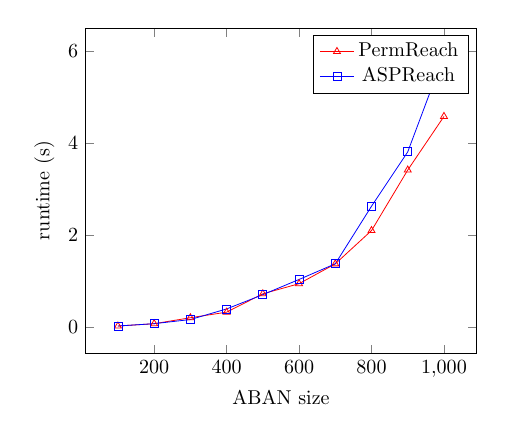
\begin{tikzpicture}[scale=0.725]
    \begin{axis}[xlabel=ABAN size,ylabel=runtime (s)]
       \addplot[mark=triangle,color=red] coordinates{
        (100,0.029)
        (200,0.079)
        (300,0.209)
        (400,0.330)
        (500,0.729)
        (600,0.948)
        (700,1.379)
        (800,2.102)
        (900,3.416)
        (1000,4.58)
        };
        \addlegendentry{PermReach}
       \addplot[mark=square,color=blue] coordinates{
        (100,0.03)
        (200,0.08)
        (300,0.17)
        (400,0.40)
        (500,0.71)
        (600,1.04)
        (700,1.38)
        (800,2.63)
        (900,3.81)
        (1000,5.91)       
        };
        \addlegendentry{ASPReach}
    \end{axis}
\end{tikzpicture}
    \label{fig:sizeTest}
    }
    \subfigure[0.5\textwidth][Average runtime(s) w.r.t. ABAN density, ABAN size fixed to 20]{
        \centering
    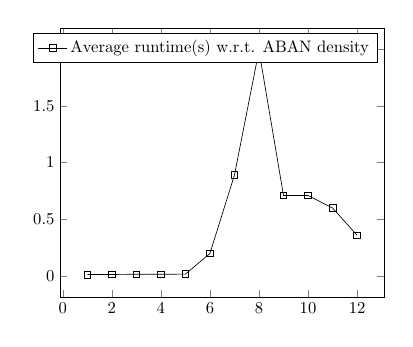
\begin{tikzpicture}[>=stealth,scale=0.6,line width=0.8pt,align=center]
    \begin{axis}%[legend pos=north west]
       \addplot[mark=square] coordinates{
(1,0.014)
(2,0.015)
(3,0.017)
(4,0.017)
(5,0.018)
(6,0.2)
(7,0.89)
(8,1.987)
(9,0.710)
(10,0.71)
(11,0.6)
(12,0.36)    
        %(1,3.57/400)
        %(2,3.9/400)
        %(3,10.4/400)
        %(4,29.4/400)
        %(5,205/400)
        %(6,275/400)
        %(7,1265/400)
        };
        \addlegendentry{Average runtime(s) w.r.t. ABAN density}
    \end{axis}
\end{tikzpicture}

    \label{fig:inconcTest}
    }
    \caption[Runtime tests of reachability analyzers]{Runtime of PermReach and ASPReach on random ABANs}
\end{figure}

\section{TBA, waiting for the collaboration with LFIT}
Random ABANs, generate time series data, hide randomly a part of transitions, calculate the percentage of retrieval

\section{R\'esum\'e}